\section{Introduction}
\subsection{Background}
\begin{frame}{Introduction}
\framesubtitle{Vision-Language Models (VLMs)}
  \begin{itemize}
    \item Neural networks that process both \emph{images} and \emph{text}
    \item Like Large Language Models (LLMs):
    \begin{itemize}
      \item Learn \emph{general visual-textual understanding} from pre-training~\footfullciteieee{Radford2021}
      \item Then aligned to human preferences and \emph{instruction-following}
    \end{itemize}
    \item Shown to be able to \emph{adapt} to new tasks without extensive task-specific training~\footfullciteieee{Liu2023}, hence quite \emph{generalizable}
    \blfootnote{\vspace{0.05em}}
  \end{itemize}
\end{frame}
\note{
- I know that most of you are already familiar with multi-modal models, being in a room of researchers in multimodal foundation models, but perhaps there are people in the audience who are not familiar with the field. So we start with a brief introduction to some concepts we will be needing today \\ 
- VLMs combine computer vision and natural language processing capabilities in a single neural network \\
- Pre-training occurs on web-scale image-text datasets (e.g., CLIP was trained on 400M image-text pairs). In this way, models learn to understand the relationship between images and text and also predict one from the other \\
- Unlike traditional CV models trained for specific tasks, VLMs learn broader understanding that transfers to many tasks \\
- Similar to how ChatGPT can answer questions on many topics, VLMs can handle multiple visual tasks \\
}


\begin{frame}{Introduction}
\framesubtitle{Few-Shot Transfer}
  \vspace{-1em}
  \begin{itemize}
    \item Teaching a \emph{generalizable model} new tasks by showing it a few \emph{examples}
    \item Model `learns' to recognize patterns from these examples
    \item Can then apply this `learning' to new, unseen instances
  \end{itemize}
  \vspace{-0.2em}
  \begin{columns}[onlytextwidth]
    \column{.5\textwidth}
    % \centering 
    \small{\emph{Prompt}: A [DOG] has droopy ears and is often fluffy. This is a [DOG]:}
    \begin{figure}
      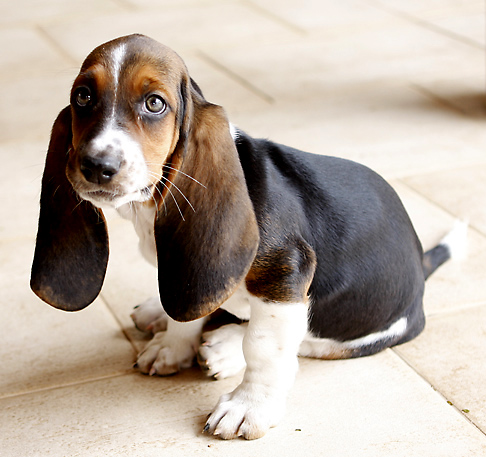
\includegraphics[width=20mm]{./figures/basset-hound.jpeg}
      \caption{\centering This is a [DOG]. \\ \tiny{Image from Wikipedia, \href{https://commons.wikimedia.org/w/index.php?curid=32270218}{Link}}}
    \end{figure}
    \column{.5\textwidth} 
    \begin{figure}
      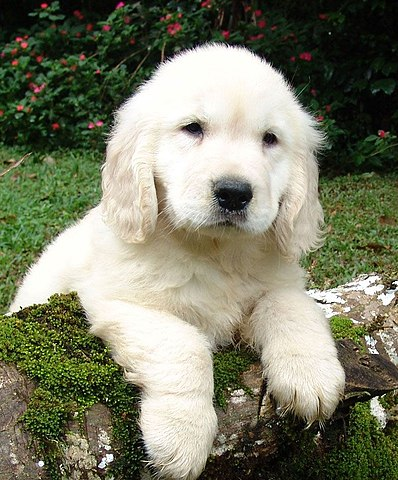
\includegraphics[width=20mm]{./figures/golden-retriever-puppy.jpeg}
      \caption{\centering Is this a [DOG]? \\ \tiny{Image from Wikipedia, \href{https://commons.wikimedia.org/w/index.php?curid=18521767}{Link}}}
    \end{figure}
    \vspace{-0.5cm}
    % \centering 
    \small{\emph{Prompt}: Is this a [DOG]?\\
    \emph{Expected Answer}: Yes}
  \end{columns}
\end{frame}
\note{
- Few-shot transfer is different from traditional machine learning that requires many examples \\
- The model doesn't actually learn in the traditional sense; it leverages knowledge from pre-training \\
- In this example, we show the model one example of a dog (a basset hound) and ask it to identify another dog \\
- This works because the model already knows what dogs look like from pre-training \\
- The quotation marks around 'learns' emphasize that it's not learning from scratch. I like to think of it as somehow narrowing the tree of possible responses from a point \\
}


% \subsection{Motivation}
\begin{frame}{Motivation}
\framesubtitle{Few-Shot Transfer}
  \vspace{-1em}
  \begin{columns}[T]
    \column{0.5\textwidth}
      \centering \emph{Fine-tuning}
      \begin{itemize}
        \item Requires significant computational resources, modifies model parameters
        \item Needs \emph{large(r) amounts} of \emph{labeled data}
        \item Can lead to catastrophic forgetting
        \item Refers to fine-tuning a pre-trained / instruction-tuned model on a specific task
      \end{itemize}
    \column{0.5\textwidth}
    \centering \emph{Few-shot Transfer}
    \begin{itemize}
        \item Uses \emph{`few' examples} or natural language \emph{descriptions}
        \item No model parameters are updated
        \item Potentially more practical for real-world applications~\footfullciteieee{Brown2020}
        \item Can be less effective for complex tasks
    \end{itemize}
  \end{columns}
\end{frame}
\note{
- Fine-tuning is the traditional approach for adapting pre-trained models to new tasks \\
- For VLMs, fine-tuning can require multiple high-end GPUs and days of compute time \\
- Catastrophic forgetting means the model may lose previously learned capabilities \\
- Few-shot transfer is much more efficient - we can use the model "as is" \\
- An important distinction: fine-tuning modifies the model weights, few-shot transfer doesn't \\
- The trade-off is that few-shot performance may not match fine-tuned performance for complex tasks \\
}


\subsection{Problem Statement}
\begin{frame}{Problem Statement}
\framesubtitle{Dataset Labeling for Computer Vision Tasks}
  \textbf{Challenge:} Creating labeled datasets to train specialized models for computer vision tasks is \emph{time-consuming} and \emph{expensive}~\footfullciteieee{Deng2009}, but VLMs are generalizable
  \vspace{0.5em}

  \textbf{Constraint:} However, VLMs are too \emph{computationally intensive} for direct deployment on resource-constrained environments (e.g., robots)
  \vspace{0.5em}
    
  \textbf{Opportunity:} VLMs could potentially automate label generation (\emph{pseudolabels}) to train \emph{downstream} models
  \vspace{1.2em}

  \centering \textbf{Research Question:} Can VLMs be transferred to generate \emph{pseudolabels} for computer vision tasks to train \emph{lightweight} downstream models?
  \blfootnote{\vspace{0.05em}}
\end{frame}
\note{
- The annotation of the ImageNet dataset required crowdsourcing to be feasible \\
- Specialized datasets like medical imaging can be even more expensive and require expert annotators \\
- VLMs require significant computational resources - multiple high-end GPUs with significant amounts of memory \\
- Most robots have limited computational capabilities - often a single low-power GPU or CPU \\
- Pseudolabels are automatically generated annotations that can be used in place of human-created labels \\
- The key insight: we don't need to deploy the large model - we use it to train a smaller, more efficient model \\
}